\documentclass[10pt]{article} % Default font size is 12pt, it can be changed here
\usepackage{amsmath}

\usepackage{geometry} % Required to change the page size to A4
\geometry{a4paper} % Set the page size to be A4 as opposed to the default US Letter

\usepackage{graphicx} % Required for including pictures

\usepackage{float} % Allows putting an [H] in \begin{figure} to specify the exact location of the figure

\linespread{1.2} % Line spacing
\graphicspath{{Pictures/}} % Specifies the directory where pictures are stored

\begin{document}

\section{Broken Symmetry} % Major section
The occurrence of a spontaneously ordered state at low temperatures is a fundamental phenomenon in solid state physics. Examples are ferromagnetism, antiferromagnetism, and superconductivity. It is characterized by the temperature dependence of the magnetization. There exists a phase transition below a critical temperature analogous to water and it's freezing temperature.

\subsection{Breaking of Symmetry}
Above a critical temperature (Curie temperature $T_C$) the system possesses a complete rotational symmetry; all directions of classical spins or magnetic moments are equivalent. Below $T_C$ a preferential alignment is present. A rotational symmetry nly occurs around the direction of magnetization; this directly proves that symmetry is broken. 

An important aspect is that the symmetry cannot be changed gradually, it happens at a specific point $T_C$.

\begin{figure}[H]
\begin{center}
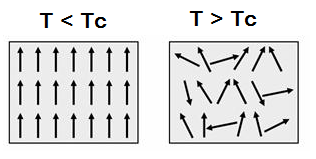
\includegraphics[scale=1.0]{curietemp}
\caption{Phase transition between the paramagnetic state $T > T_C$ and the ferromagnetic state $T < T_C$}
\end{center}
\end{figure}

\subsection{Different Models of Magnetic Behavior}
We will discuss different models which describe he order parameter magnetization $\vec{M}$ as a function of temperature T.

\subsubsection{Landau Theory}
Landau theory is a mean-field theory, thus is characterized by the assumption that all magnetic moments are inflenced by an identical averaged exchange field induced by all neighbors and is identical with the model of Weiss. The advantage of this approach using mean field theories is given by their simplicity, but correlations and fluctuations which are important are neglected near $T_C$. Therefore, results near the Cureie temperature are less confidential compared to that for low temperatures. 

The free energy of a ferromagnetic system is described by a function of the order parameter using a power series in $\vec{M}$. Both opposite magnetization states ehibit no energetic difference, i.e. they are energetically degenerated, which leads to a vanishing terms of M to the power of odd values. The free energy can then be written as:

\begin{equation}
F(M) = F_0 + a(T)M^2 + bM^4
\end{equation}

with $F_0$ being constant, $b > 0$ and constant, $a(T) = a_0(T - T_C)$ and $a_0$ being positive. From this one is able to determine the magnetization as a function of temperature by considering the minimums of the free energy with respect to the magnetization. Thus $M(T)$ is given by:

\begin{align*} 
M &= \pm \sqrt{\frac{a_0(T_C - T)}{2b}} &\text{for} \quad &T > T_C \\
M &= 0  &\text{for} \quad &T \leq T_C
\end{align*}

The behavior of the free energy F(M) is summarized in the figure.

\begin{figure}[H]
\begin{center}
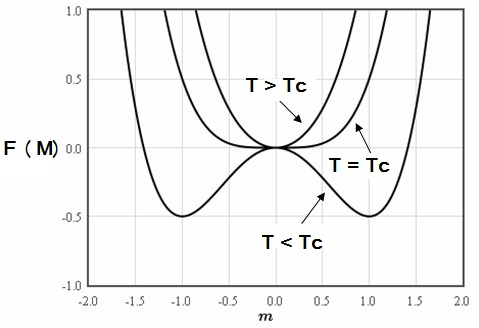
\includegraphics[scale=0.8]{freeenergy}
\caption{Free energy F(M) for temperatures below, at, and above the critical temperature $T_C$}
\end{center}
\end{figure}


\subsubsection{Heisenberg Model}
Not covered.
$\pagebreak$

\subsection{Consequences}
Important consequences of the broken symmetry are:

\begin{itemize}
\item Existence of phase transitions - A sharp transition occurs at the critical temperature (paramagnet to ferromagnet)
\item Rigidity - After breaking the symmetry the system strongly tries to remain in the actual state because changes desire energy
\item Excitations - Neglecting fluctuations due to quantum effects perfect order occurs at T = 0K. With increasing temperature the degree of ordering is decreased due to excitations concerning the order parameter. For crystal lattice vibrations can be correlated with phonons. For ferromagnets spin waves are related to magnons.
\item Defects - The broken symmetry often result in different behavior in regions being neighbored in a macroscopic system. The boundary represents a defect. In crystals the defect may be a dislocation or grain boundary. In ferromagnets it is a domain wall.
\end{itemize}

\subsection{Phase Transitions}
\underline{In the vicinity of the critical temperature} important properties can be described using an exponential function, e.g. $M \propto (T_C - T)^x$. The parameter x is called the "critical exponent". Continuous phase transitions are related to critical exponents which exclusively depend on the:

\begin{itemize}
\item dimensionality of the system d
\item dimensionality of the order parameter D
\item range of the forces being involved (long-short)
\end{itemize}

\subsubsection{Critical Exponents for Ferromagnetic Systems using Landau Theory}
The most commonly used critical exponents describing ferromagnetic systems are:

\begin{itemize}
\item $\beta$ characterizing the order parameter M for $T < T_C$:
\begin{equation}
M \propto (T_C - T)^\beta
\end{equation}
It can be found that $\beta = \frac{1}{2}$

\item $\gamma$ characterizing the susceptibility $\chi$ for $T > T_C$:
\begin{equation}
\chi \propto (T - T_C)^{-\gamma}
\end{equation}
It can be found that $\gamma = 1$

\item $\alpha$ characterizing the specific heat $c_H$ for $T > T_C$:
\begin{equation}
c_H \propto (T - T_C)^{-\alpha}
\end{equation}
It can be found that $\alpha = 0 \implies$ the specific heat $c_H$ exhibits a discontinuity at the Curie temperature.

\item $\delta$ characterizing the influence of an external magnetic field H on the magnetization M at $T = T_C$:
\begin{equation}
M \propto H^{\frac{1}{\delta}}
\end{equation}
It can be found that $\delta = 3$

\item $\nu$ characterizing the correlation length $\xi$ for $T < T_C$:
\begin{equation}
\xi \propto (T_C - T)^{-\nu}
\end{equation}
It can be found that $\nu = \frac{1}{2}$
\end{itemize}

\subsubsection{Scaling Laws}
The scaling laws describe the relationship between different critical exponents which are valid for all exactly solvable models. For each different theory(Landau, 2d-Ising, 3d-Ising, XY model, 3d-Heisenberg...) all have different critical exponents, but they all obey the scaling laws:

\begin{equation}
2 = \alpha + 2\beta + \gamma
\end{equation}
\begin{equation}
\delta = 1 + \frac{\gamma}{\beta}
\end{equation}
\begin{equation}
\alpha = 2 - d\nu
\end{equation}

The last relationship is only valid within Landau theory for $d = 4$. Additionally, we find that $\alpha, \gamma, \nu$ exhibit the same value below and above the Curie temperature which is by no means a triviality.

In the figure, one can see the different critical values for different models, yet they all obey the scaling laws.


\begin{figure}[H]
\begin{center}
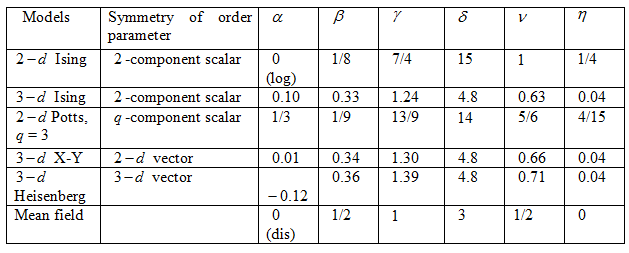
\includegraphics[scale=0.8]{critexponents}
\caption{Different critical exponents for different models}
\end{center}
\end{figure}


\subsection{Magnetic Excitations}
The description of, e.g. the magnetization $M$ as a function of temperature by exponential laws and the calculation of critical exponents $\underline{fails}$ at lower temperatures $\approx \frac{T}{T_C} < \frac{1}{2}$. Thus, another attempt must be used. 

For low temperatures the descrition is carried out using low-energetic magnetic excitations. These spin waves are quantized by magnons. An analog are lattice vibrations in crystals which are quantized by phonons. 

The dispersion relation for magnons of an isotropic ferromagnet is given by:

\begin{equation}
\hbar \omega = 4JS(1 - cosqa)
\end{equation}

This is shown in the figure. As no gap occurs at $\hbar \omega = 0$ already smallest excitation energies can create spin waves. Magnons are bosons ($1\hbar$) because every magnon represents a delocalized switched spin.
\begin{figure}[H]
\begin{center}
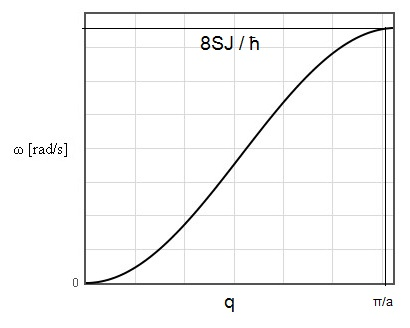
\includegraphics[scale=0.5]{magnondispersion}
\caption{Dispersion relation of a magnon in a one-dimensional chain}
\end{center}
\end{figure}

\begin{figure}[H]
\begin{center}
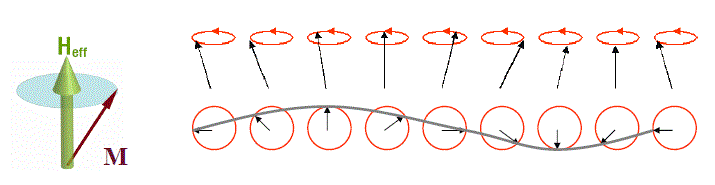
\includegraphics[scale=0.6]{spinwave2}
\caption{Spin wave of a one-atomic chain}
\end{center}
\end{figure}

\subsubsection{Magnetization Near T = 0K}
Near T = 0K, the magnetization follows the so-called Bloch-$T^{\frac{3}{2}}$ law:

\begin{equation}
\frac{M(T)}{M(0)} = 1 - acT^{\frac{3}{2}}
\end{equation}






Summarizing, the magnetization can be described near T = 0K by the Bloch-$T^{\frac{3}{2}}$ law and near the Curie temperature $T_C$ by the scaling law $(T - T_C)^{\beta}$.




\end{document}